\documentclass[letterpaper,journal]{IEEEtran}

% A classe IEEEtran define margens, fontes, colunas, títulos e legendas.
\usepackage{amsmath,amssymb,amsfonts,mathtools}
\usepackage{graphicx,array,multirow}
\usepackage{float}
\usepackage[utf8]{inputenc}
\usepackage[T1]{fontenc}
\graphicspath{ {./images/} }
\usepackage{microtype}
\usepackage{cite}
\usepackage{url}
\usepackage{tikz}
\usepackage{placeins}
\usepackage[portuguese]{babel}
\renewcommand{\IEEEkeywordsname}{Palavras-chave}


\begin{document}
% -----------------------------------------------------------
% 1. TÍTULO e 2. AUTORES 
% Título e autores no formato de periódico IEEE.
% -----------------------------------------------------------
\title{Séries de Fourier: harmônicas, energia e validação por FFT}

\author{Vitor Gabriel Saturnino de Melo - N.\textsuperscript{o} USP: 14611599\\
João Pedro Muto Cisotto - N.\textsuperscript{o} USP: 14761684\\[0.5ex]
\normalsize Departamento de Engenharia Elétrica\\
\normalsize Lista T1 --- 2026}

\markboth{Departamento de Engenharia Elétrica --- Lista T1 --- 2026}%
{Séries de Fourier: harmônicas, energia e validação por FFT}

\maketitle
% Mantém o espaçamento natural quando um elemento [H] passa à coluna seguinte.
\raggedbottom





% ==========================================
% SEÇÕES INICIAIS
% ==========================================

% 3. Resumo
\begin{abstract}
Nesta tarefa, discutirá-se definições e conceitos relacionados à transformada Z e à estabilidade de sistemas. Para isso, será realizada a análise de dois sistemas para verificar os teoremas abordados em aula, além de obter a distribuição da saída em resposta ao degrau unitário, obtendo, assim, um gráfico da resposta no domínio ‘k’ além da obtenção do comportamento do sistema.
\end{abstract}

%\keywords{Keywords}


% 4. Introdução
\section{Introdução}

\IEEEPARstart{A}{} série de Fourier representa um sinal periódico como a soma de uma
componente contínua e de senos e cossenos em múltiplos da frequência
fundamental. Essa decomposição permite reconstruir formas de onda,
comparar seu conteúdo espectral e quantificar a contribuição energética
de cada harmônico.

Para comprovar esse comportamento, serão utilizados diversos sinais e calculados
suas representações em série de Fourier e sua energia. O desenvolvimento
preserva as amplitudes e os intervalos como variáveis e apresenta as
integrais e suas simplificações. Em seguida, trata os deslocamentos e a
mudança do período, calcula as energias por Parseval e compara os
resultados com a FFT. 



% 5. Definição do Problema
%\section{Definição do problema}

O enunciado reproduzido no memorial solicita as equações das oito ondas
da Figura 1 e das seis variações da Figura 2, até a ordem harmônica 7,
uma comparação teórica com FFT no MATLAB/Simulink e as energias da
fundamental e das sete primeiras ordens em relação ao sinal completo.
Para as retangulares, devem ser contemplados $\phi=\theta$ e
$\phi\neq\theta$; para as ondas deslocadas, $\delta=P$ e $\delta\neq P$.

Adota-se $x=\omega t$, com $\omega>0$ em rad/s e amplitude $A>0$ em V.
O intervalo angular nominal é $P=\omega T$. O período angular efetivo
será indicado por $L$: $L=P$ nos ciclos simples, $L=\delta$ nas ondas
da Figura 2 e $L=2P$ na alternância de dois ciclos retangulares distintos.
O período físico e a frequência fundamental são, portanto,
\begin{equation}
    T_0=\frac{L}{\omega}, \qquad f_0=\frac{1}{T_0}=\frac{\omega}{L}.
\end{equation}

Para evitar a ambiguidade do símbolo $\delta$, a largura do pulso
retangular da Figura 1 será escrita como $d$, enquanto $\delta$ denotará
o período efetivo da Figura 2. Os intervalos $\phi$ e $\theta$ são
medidas angulares antes e depois do pulso, e não amplitudes.

Uma onda periódica não nula tem energia infinita quando integrada em
todo o eixo temporal. Neste trabalho, ``energia do sinal completo''
significa a integral de seu quadrado em um período, incluindo a
componente contínua. A energia apenas das ordens 1 a 7 será distinguida
da energia da reconstrução que também inclui a média.
 % Renomeie seu arquivo "Desenvolvimento.tex" para "definicao_problema.tex" ou altere aqui


% ==========================================
% DESENVOLVIMENTO, RESULTADOS E CONCLUSÃO
% ==========================================

% 6. Solução do Problema
\section{Desenvolvimento}
\label{Desenvolvimento}
\subsection{Sinal 1: rampa crescente de 0 a A}:

\begin{figure}[H]
    \centering
    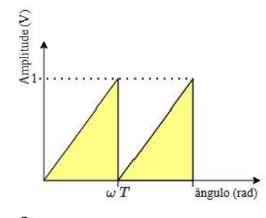
\includegraphics[width=0.6\linewidth]{images/rampa_crescente.png}
    \caption{Sinal de entrada rampa crescente de 0 a P}
    \label{fig:sinal1}
\end{figure}

Para o sinal de entrada rampa crescente de 0 a A, ela pode ser representada por
uma reta que liga o ponto (0,0) ao ponto (P,A). Seu coeficiente angular é dado 
por $\frac{A}{P}$, e a equação da reta é dada por:

\begin{equation}
    v_1(x) = \frac{A}{P}x, 0\leq x < P, v_1(x+P)= v_1(x)
\end{equation}

O valor médio dessa função pode ser calculado pela integral da função em um 
período, dividida pelo período, dessa forma, pode-se calcular esse valor com a 
equação abaixo: 

\begin{equation}
    a_0 = \frac{1}{P} \int_{0}^{P} v_1(x) dx = \frac{1}{P} \int_{0}^{P} \frac{A}{P}x dx = \frac{A}{2}
\end{equation}

Ademais, para construir sua representação em série de Fourier, é necessário 
calcular os coeficientes $a_n$ e $b_n$, que são dados pelas equações abaixo:

\begin{equation}
    \begin{aligned}
        a_n &= \frac{2}{P} \int_{0}^{P} v_1(x)
            \cos\left(\frac{2\pi nx}{P}\right)\,dx \\
            &= \frac{2A}{P^2} \int_{0}^{P} x
            \cos\left(\frac{2\pi nx}{P}\right)\,dx \\
            &= \frac{2A}{P^2} \left[
            \frac{Px}{2\pi n}\sin\left(\frac{2\pi nx}{P}\right)\right. \\
            &\qquad \left.{}+ \frac{P^2}{4\pi^2 n^2}
            \cos\left(\frac{2\pi nx}{P}\right)\right]_{0}^{P} \\
            &= \frac{2A}{P^2} \left[
            \frac{P^2}{4\pi^2 n^2}\cos(2\pi n)
            - \frac{P^2}{4\pi^2 n^2}\cos(0)\right] \\
            &= 0.
    \end{aligned}
\end{equation}


% 7. Resultados de Implementação
\FloatBarrier
\raggedbottom
\section{Resultados}
A comparação abrange as seis ondas básicas da Figura 1,
as seis ondas da Figura 2 em cada condição $\delta=P$ e
$\delta=0{,}8P$, com $\phi=P/10$, e as duas retangulares
nos casos simétrico, assimétrico e alternado. Os 24 cenários
têm seus coeficientes, energias e gráficos apresentados a seguir.

\subsection{Grandezas extraídas da simulação}
Sejam $y_j$ as amostras simuladas. A FFT normalizada e a correção
para o início em meia amostra são
\begin{equation}
    \begin{aligned}
        Y_n&=\frac1N\sum_{j=0}^{N-1}y_j
            \exp\left(-\mathrm{i}\frac{2\pi nj}{N}\right), \\
        \widehat c_n&=Y_n\exp\left(-\mathrm{i}\frac{\pi n}{N}\right), \\
        \widehat a_0&=\operatorname{Re}(Y_0), \\
        \widehat a_n&=2\operatorname{Re}(\widehat c_n), \qquad
        \widehat b_n=-2\operatorname{Im}(\widehat c_n), \\
        \widehat C_n&=\sqrt{\widehat a_n^2+\widehat b_n^2}.
    \end{aligned}
\end{equation}
A energia total simulada é estimada diretamente pelas amostras;
as energias das ordens 1 a 7 utilizam os coeficientes medidos pela FFT:
\begin{equation}
    \begin{aligned}
        \widehat E_L^{(x)}&=\frac LN\sum_{j=0}^{N-1}y_j^2, \\
        \widehat E_{\mathrm{CC}}&=L\widehat a_0^2, \qquad
        \widehat E_1=\frac L2\widehat C_1^2, \\
        \widehat E_{1:7}&=\frac L2\sum_{n=1}^{7}\widehat C_n^2, \\
        \widehat E_{\mathrm{CC}:7}&=\widehat E_{\mathrm{CC}}+\widehat E_{1:7}.
    \end{aligned}
\end{equation}

Cada percentual simulado é calculado dividindo a energia estimada
da parcela pela energia total estimada $\widehat E_L^{(x)}$.
Os valores teóricos usam as integrais e os coeficientes analíticos,
com seus próprios denominadores.

\subsection{Média e amplitude da fundamental}

Foram simulados 24 cenários, com $N=65536$ amostras por período real.
 As tabelas apresentam lado a lado os valores da teoria (T) e da simulação (S).
  Os valores S foram obtidos aplicando a FFT do MATLAB às amostras geradas.

Nas tabelas, S1 a S6 identificam as seis formas de onda já definidas;
as abreviações \textit{uni.} e \textit{bi.} indicam retangulares
unipolares e bipolares, e \textit{sim.}, \textit{assim.} e \textit{alt.}
seus casos simétrico, assimétrico e alternado, respectivamente.
Os cabeçalhos T e S indicam teoria e simulação.

\begin{table}[H]
\centering\small
\setlength{\tabcolsep}{3.5pt}
\caption{Ondas básicas: média e amplitude da fundamental em V.}\label{tab:fft}
\begin{tabular}{lrrrr}\hline
Caso & $a_{0,\mathrm T}$ & $a_{0,\mathrm S}$ & $C_{1,\mathrm T}$ & $C_{1,\mathrm S}$ \\ \hline
S1 & $0{,}500000$ & $0{,}500000$ & $0{,}318310$ & $0{,}318310$ \\
S2 & $0{,}500000$ & $0{,}500000$ & $0{,}318310$ & $0{,}318310$ \\
S3 & $0{,}500000$ & $0{,}500000$ & $0{,}405285$ & $0{,}405285$ \\
S4 & $0{,}000000$ & $0{,}000000$ & $0{,}636620$ & $0{,}636620$ \\
S5 & $0{,}000000$ & $0{,}000000$ & $0{,}636620$ & $0{,}636620$ \\
S6 & $0{,}000000$ & $0{,}000000$ & $0{,}810569$ & $0{,}810569$ \\
\hline\end{tabular}
\end{table}
\begin{table}[H]
\centering\small
\setlength{\tabcolsep}{3.5pt}
\caption{Ondas deslocadas com $\delta=P$: média e fundamental em V.}\label{tab:fft_P}
\begin{tabular}{lrrrr}\hline
Caso & $a_{0,\mathrm T}$ & $a_{0,\mathrm S}$ & $C_{1,\mathrm T}$ & $C_{1,\mathrm S}$ \\ \hline
S1 & $0{,}500000$ & $0{,}500006$ & $0{,}318310$ & $0{,}318310$ \\
S2 & $0{,}500000$ & $0{,}499994$ & $0{,}318310$ & $0{,}318310$ \\
S3 & $0{,}500000$ & $0{,}500000$ & $0{,}405285$ & $0{,}405285$ \\
S4 & $0{,}000000$ & $0{,}000012$ & $0{,}636620$ & $0{,}636620$ \\
S5 & $0{,}000000$ & $-0{,}000012$ & $0{,}636620$ & $0{,}636620$ \\
S6 & $0{,}000000$ & $0{,}000000$ & $0{,}810569$ & $0{,}810569$ \\
\hline\end{tabular}
\end{table}
\begin{table}[H]
\centering\small
\setlength{\tabcolsep}{3.5pt}
\caption{Ondas deslocadas com $\delta=0{,}8P$: média e fundamental em V.}\label{tab:fft_08P}
\begin{tabular}{lrrrr}\hline
Caso & $a_{0,\mathrm T}$ & $a_{0,\mathrm S}$ & $C_{1,\mathrm T}$ & $C_{1,\mathrm S}$ \\ \hline
S1 & $0{,}500000$ & $0{,}500000$ & $0{,}318310$ & $0{,}318310$ \\
S2 & $0{,}500000$ & $0{,}500000$ & $0{,}318310$ & $0{,}318310$ \\
S3 & $0{,}500000$ & $0{,}500000$ & $0{,}405285$ & $0{,}405285$ \\
S4 & $0{,}000000$ & $0{,}000000$ & $0{,}636620$ & $0{,}636620$ \\
S5 & $0{,}000000$ & $0{,}000000$ & $0{,}636620$ & $0{,}636620$ \\
S6 & $0{,}000000$ & $0{,}000000$ & $0{,}810569$ & $0{,}810569$ \\
\hline\end{tabular}
\end{table}
\begin{table}[H]
\centering\small
\setlength{\tabcolsep}{3.5pt}
\caption{Retangulares: média e amplitude da fundamental em V.}\label{tab:fft_ret}
\begin{tabular}{lrrrr}\hline
Caso & $a_{0,\mathrm T}$ & $a_{0,\mathrm S}$ & $C_{1,\mathrm T}$ & $C_{1,\mathrm S}$ \\ \hline
Uni. sim. & $0{,}333333$ & $0{,}333344$ & $0{,}551329$ & $0{,}551339$ \\
Uni. assim. & $0{,}333333$ & $0{,}333328$ & $0{,}551329$ & $0{,}551324$ \\
Uni. alt. & $0{,}416667$ & $0{,}416672$ & $0{,}236174$ & $0{,}236177$ \\
Bi. sim. & $-0{,}333333$ & $-0{,}333313$ & $1{,}102658$ & $1{,}102678$ \\
Bi. assim. & $-0{,}333333$ & $-0{,}333344$ & $1{,}102658$ & $1{,}102648$ \\
Bi. alt. & $-0{,}166667$ & $-0{,}166656$ & $0{,}472349$ & $0{,}472353$ \\
\hline\end{tabular}
\end{table}


As Tabelas \ref{tab:fft}--\ref{tab:fft_ret} mostram a preservação
da amplitude da fundamental após deslocar ou mudar o período das
seis ondas. Nas retangulares, os valores simulados também reproduzem
a igualdade de $C_1$ entre os pulsos simétrico e assimétrico de mesmo
$D$. Na alternância, a fundamental passa a corresponder ao período
$2P$, e sua amplitude é diferente da de um pulso de período $P$.

\subsection{Coeficientes das ordens 1 a 7}
As Tabelas \ref{tab:coef_comp1}--\ref{tab:coef_comp24} apresentam
os sete pares $(a_n,b_n)$ de todos os 24 cenários, com teoria e
FFT lado a lado. A ordem é: seis sinais básicos, seis deslocados
com $\delta=P$, seis com $\delta=0{,}8P$ e seis retangulares.
Estão incluídas todas as rampas crescentes e decrescentes,
os triângulos e as variantes unipolares e bipolares.

\begin{table}[H]
\centering\small
\setlength{\tabcolsep}{3.5pt}
\caption{Rampa crescente uni.: coeficientes em V, teoria (T) e FFT da simulação (S).}\label{tab:coef_comp1}
\begin{tabular}{crrrr}\hline
$n$ & $a_{n,\mathrm T}$ & $a_{n,\mathrm S}$ & $b_{n,\mathrm T}$ & $b_{n,\mathrm S}$ \\ \hline
1 & $0{,}000000$ & $0{,}000000$ & $-0{,}318310$ & $-0{,}318310$ \\
2 & $0{,}000000$ & $0{,}000000$ & $-0{,}159155$ & $-0{,}159155$ \\
3 & $0{,}000000$ & $0{,}000000$ & $-0{,}106103$ & $-0{,}106103$ \\
4 & $0{,}000000$ & $0{,}000000$ & $-0{,}079577$ & $-0{,}079577$ \\
5 & $0{,}000000$ & $0{,}000000$ & $-0{,}063662$ & $-0{,}063662$ \\
6 & $0{,}000000$ & $0{,}000000$ & $-0{,}053052$ & $-0{,}053052$ \\
7 & $0{,}000000$ & $0{,}000000$ & $-0{,}045473$ & $-0{,}045473$ \\
\hline\end{tabular}
\end{table}
\begin{table}[H]
\centering\small
\setlength{\tabcolsep}{3.5pt}
\caption{Rampa decrescente uni.: coeficientes em V, teoria (T) e FFT da simulação (S).}\label{tab:coef_comp2}
\begin{tabular}{crrrr}\hline
$n$ & $a_{n,\mathrm T}$ & $a_{n,\mathrm S}$ & $b_{n,\mathrm T}$ & $b_{n,\mathrm S}$ \\ \hline
1 & $0{,}000000$ & $0{,}000000$ & $0{,}318310$ & $0{,}318310$ \\
2 & $0{,}000000$ & $0{,}000000$ & $0{,}159155$ & $0{,}159155$ \\
3 & $0{,}000000$ & $0{,}000000$ & $0{,}106103$ & $0{,}106103$ \\
4 & $0{,}000000$ & $0{,}000000$ & $0{,}079577$ & $0{,}079577$ \\
5 & $0{,}000000$ & $0{,}000000$ & $0{,}063662$ & $0{,}063662$ \\
6 & $0{,}000000$ & $0{,}000000$ & $0{,}053052$ & $0{,}053052$ \\
7 & $0{,}000000$ & $0{,}000000$ & $0{,}045473$ & $0{,}045473$ \\
\hline\end{tabular}
\end{table}
\begin{table}[H]
\centering\small
\setlength{\tabcolsep}{3.5pt}
\caption{Triangular uni.: coeficientes em V, teoria (T) e FFT da simulação (S).}\label{tab:coef_comp3}
\begin{tabular}{crrrr}\hline
$n$ & $a_{n,\mathrm T}$ & $a_{n,\mathrm S}$ & $b_{n,\mathrm T}$ & $b_{n,\mathrm S}$ \\ \hline
1 & $-0{,}405285$ & $-0{,}405285$ & $0{,}000000$ & $0{,}000000$ \\
2 & $0{,}000000$ & $0{,}000000$ & $0{,}000000$ & $0{,}000000$ \\
3 & $-0{,}045032$ & $-0{,}045032$ & $0{,}000000$ & $0{,}000000$ \\
4 & $0{,}000000$ & $0{,}000000$ & $0{,}000000$ & $0{,}000000$ \\
5 & $-0{,}016211$ & $-0{,}016211$ & $0{,}000000$ & $0{,}000000$ \\
6 & $0{,}000000$ & $0{,}000000$ & $0{,}000000$ & $0{,}000000$ \\
7 & $-0{,}008271$ & $-0{,}008271$ & $0{,}000000$ & $0{,}000000$ \\
\hline\end{tabular}
\end{table}
\begin{table}[H]
\centering\small
\setlength{\tabcolsep}{3.5pt}
\caption{Rampa crescente bi.: coeficientes em V, teoria (T) e FFT da simulação (S).}\label{tab:coef_comp4}
\begin{tabular}{crrrr}\hline
$n$ & $a_{n,\mathrm T}$ & $a_{n,\mathrm S}$ & $b_{n,\mathrm T}$ & $b_{n,\mathrm S}$ \\ \hline
1 & $0{,}000000$ & $0{,}000000$ & $-0{,}636620$ & $-0{,}636620$ \\
2 & $0{,}000000$ & $0{,}000000$ & $-0{,}318310$ & $-0{,}318310$ \\
3 & $0{,}000000$ & $0{,}000000$ & $-0{,}212207$ & $-0{,}212207$ \\
4 & $0{,}000000$ & $0{,}000000$ & $-0{,}159155$ & $-0{,}159155$ \\
5 & $0{,}000000$ & $0{,}000000$ & $-0{,}127324$ & $-0{,}127324$ \\
6 & $0{,}000000$ & $0{,}000000$ & $-0{,}106103$ & $-0{,}106103$ \\
7 & $0{,}000000$ & $0{,}000000$ & $-0{,}090946$ & $-0{,}090946$ \\
\hline\end{tabular}
\end{table}
\begin{table}[H]
\centering\small
\setlength{\tabcolsep}{3.5pt}
\caption{Rampa decrescente bi.: coeficientes em V, teoria (T) e FFT da simulação (S).}\label{tab:coef_comp5}
\begin{tabular}{crrrr}\hline
$n$ & $a_{n,\mathrm T}$ & $a_{n,\mathrm S}$ & $b_{n,\mathrm T}$ & $b_{n,\mathrm S}$ \\ \hline
1 & $0{,}000000$ & $0{,}000000$ & $0{,}636620$ & $0{,}636620$ \\
2 & $0{,}000000$ & $0{,}000000$ & $0{,}318310$ & $0{,}318310$ \\
3 & $0{,}000000$ & $0{,}000000$ & $0{,}212207$ & $0{,}212207$ \\
4 & $0{,}000000$ & $0{,}000000$ & $0{,}159155$ & $0{,}159155$ \\
5 & $0{,}000000$ & $0{,}000000$ & $0{,}127324$ & $0{,}127324$ \\
6 & $0{,}000000$ & $0{,}000000$ & $0{,}106103$ & $0{,}106103$ \\
7 & $0{,}000000$ & $0{,}000000$ & $0{,}090946$ & $0{,}090946$ \\
\hline\end{tabular}
\end{table}
\begin{table}[H]
\centering\small
\setlength{\tabcolsep}{3.5pt}
\caption{Triangular bi.: coeficientes em V, teoria (T) e FFT da simulação (S).}\label{tab:coef_comp6}
\begin{tabular}{crrrr}\hline
$n$ & $a_{n,\mathrm T}$ & $a_{n,\mathrm S}$ & $b_{n,\mathrm T}$ & $b_{n,\mathrm S}$ \\ \hline
1 & $-0{,}810569$ & $-0{,}810569$ & $0{,}000000$ & $0{,}000000$ \\
2 & $0{,}000000$ & $0{,}000000$ & $0{,}000000$ & $0{,}000000$ \\
3 & $-0{,}090063$ & $-0{,}090063$ & $0{,}000000$ & $0{,}000000$ \\
4 & $0{,}000000$ & $0{,}000000$ & $0{,}000000$ & $0{,}000000$ \\
5 & $-0{,}032423$ & $-0{,}032423$ & $0{,}000000$ & $0{,}000000$ \\
6 & $0{,}000000$ & $0{,}000000$ & $0{,}000000$ & $0{,}000000$ \\
7 & $-0{,}016542$ & $-0{,}016542$ & $0{,}000000$ & $0{,}000000$ \\
\hline\end{tabular}
\end{table}
\begin{table}[H]
\centering\small
\setlength{\tabcolsep}{3.5pt}
\caption{Rampa crescente uni., $\delta=P$, $\phi=P/10$: coeficientes em V, teoria (T) e FFT da simulação (S).}\label{tab:coef_comp7}
\begin{tabular}{crrrr}\hline
$n$ & $a_{n,\mathrm T}$ & $a_{n,\mathrm S}$ & $b_{n,\mathrm T}$ & $b_{n,\mathrm S}$ \\ \hline
1 & $0{,}187098$ & $0{,}187108$ & $-0{,}257518$ & $-0{,}257511$ \\
2 & $0{,}151365$ & $0{,}151369$ & $-0{,}049182$ & $-0{,}049170$ \\
3 & $0{,}100910$ & $0{,}100906$ & $0{,}032788$ & $0{,}032799$ \\
4 & $0{,}046774$ & $0{,}046765$ & $0{,}064380$ & $0{,}064387$ \\
5 & $0{,}000000$ & $-0{,}000012$ & $0{,}063662$ & $0{,}063662$ \\
6 & $-0{,}031183$ & $-0{,}031193$ & $0{,}042920$ & $0{,}042913$ \\
7 & $-0{,}043247$ & $-0{,}043251$ & $0{,}014052$ & $0{,}014040$ \\
\hline\end{tabular}
\end{table}
\begin{table}[H]
\centering\small
\setlength{\tabcolsep}{3.5pt}
\caption{Rampa decrescente uni., $\delta=P$, $\phi=P/10$: coeficientes em V, teoria (T) e FFT da simulação (S).}\label{tab:coef_comp8}
\begin{tabular}{crrrr}\hline
$n$ & $a_{n,\mathrm T}$ & $a_{n,\mathrm S}$ & $b_{n,\mathrm T}$ & $b_{n,\mathrm S}$ \\ \hline
1 & $-0{,}187098$ & $-0{,}187108$ & $0{,}257518$ & $0{,}257511$ \\
2 & $-0{,}151365$ & $-0{,}151369$ & $0{,}049182$ & $0{,}049170$ \\
3 & $-0{,}100910$ & $-0{,}100906$ & $-0{,}032788$ & $-0{,}032799$ \\
4 & $-0{,}046774$ & $-0{,}046765$ & $-0{,}064380$ & $-0{,}064387$ \\
5 & $0{,}000000$ & $0{,}000012$ & $-0{,}063662$ & $-0{,}063662$ \\
6 & $0{,}031183$ & $0{,}031193$ & $-0{,}042920$ & $-0{,}042913$ \\
7 & $0{,}043247$ & $0{,}043251$ & $-0{,}014052$ & $-0{,}014040$ \\
\hline\end{tabular}
\end{table}
\begin{table}[H]
\centering\small
\setlength{\tabcolsep}{3.5pt}
\caption{Triangular uni., $\delta=P$, $\phi=P/10$: coeficientes em V, teoria (T) e FFT da simulação (S).}\label{tab:coef_comp9}
\begin{tabular}{crrrr}\hline
$n$ & $a_{n,\mathrm T}$ & $a_{n,\mathrm S}$ & $b_{n,\mathrm T}$ & $b_{n,\mathrm S}$ \\ \hline
1 & $-0{,}327882$ & $-0{,}327882$ & $-0{,}238220$ & $-0{,}238220$ \\
2 & $0{,}000000$ & $0{,}000000$ & $0{,}000000$ & $0{,}000000$ \\
3 & $0{,}013916$ & $0{,}013916$ & $-0{,}042828$ & $-0{,}042828$ \\
4 & $0{,}000000$ & $0{,}000000$ & $0{,}000000$ & $0{,}000000$ \\
5 & $0{,}016211$ & $0{,}016211$ & $0{,}000000$ & $0{,}000000$ \\
6 & $0{,}000000$ & $0{,}000000$ & $0{,}000000$ & $0{,}000000$ \\
7 & $0{,}002556$ & $0{,}002556$ & $0{,}007866$ & $0{,}007866$ \\
\hline\end{tabular}
\end{table}
\begin{table}[H]
\centering\small
\setlength{\tabcolsep}{3.5pt}
\caption{Rampa crescente bi., $\delta=P$, $\phi=P/10$: coeficientes em V, teoria (T) e FFT da simulação (S).}\label{tab:coef_comp10}
\begin{tabular}{crrrr}\hline
$n$ & $a_{n,\mathrm T}$ & $a_{n,\mathrm S}$ & $b_{n,\mathrm T}$ & $b_{n,\mathrm S}$ \\ \hline
1 & $0{,}374196$ & $0{,}374215$ & $-0{,}515036$ & $-0{,}515022$ \\
2 & $0{,}302731$ & $0{,}302738$ & $-0{,}098363$ & $-0{,}098340$ \\
3 & $0{,}201820$ & $0{,}201813$ & $0{,}065575$ & $0{,}065599$ \\
4 & $0{,}093549$ & $0{,}093529$ & $0{,}128759$ & $0{,}128773$ \\
5 & $0{,}000000$ & $-0{,}000024$ & $0{,}127324$ & $0{,}127324$ \\
6 & $-0{,}062366$ & $-0{,}062386$ & $0{,}085839$ & $0{,}085825$ \\
7 & $-0{,}086494$ & $-0{,}086502$ & $0{,}028104$ & $0{,}028081$ \\
\hline\end{tabular}
\end{table}
\begin{table}[H]
\centering\small
\setlength{\tabcolsep}{3.5pt}
\caption{Rampa decrescente bi., $\delta=P$, $\phi=P/10$: coeficientes em V, teoria (T) e FFT da simulação (S).}\label{tab:coef_comp11}
\begin{tabular}{crrrr}\hline
$n$ & $a_{n,\mathrm T}$ & $a_{n,\mathrm S}$ & $b_{n,\mathrm T}$ & $b_{n,\mathrm S}$ \\ \hline
1 & $-0{,}374196$ & $-0{,}374215$ & $0{,}515036$ & $0{,}515022$ \\
2 & $-0{,}302731$ & $-0{,}302738$ & $0{,}098363$ & $0{,}098340$ \\
3 & $-0{,}201820$ & $-0{,}201813$ & $-0{,}065575$ & $-0{,}065599$ \\
4 & $-0{,}093549$ & $-0{,}093529$ & $-0{,}128759$ & $-0{,}128773$ \\
5 & $0{,}000000$ & $0{,}000024$ & $-0{,}127324$ & $-0{,}127324$ \\
6 & $0{,}062366$ & $0{,}062386$ & $-0{,}085839$ & $-0{,}085825$ \\
7 & $0{,}086494$ & $0{,}086502$ & $-0{,}028104$ & $-0{,}028081$ \\
\hline\end{tabular}
\end{table}
\begin{table}[H]
\centering\small
\setlength{\tabcolsep}{3.5pt}
\caption{Triangular bi., $\delta=P$, $\phi=P/10$: coeficientes em V, teoria (T) e FFT da simulação (S).}\label{tab:coef_comp12}
\begin{tabular}{crrrr}\hline
$n$ & $a_{n,\mathrm T}$ & $a_{n,\mathrm S}$ & $b_{n,\mathrm T}$ & $b_{n,\mathrm S}$ \\ \hline
1 & $-0{,}655764$ & $-0{,}655764$ & $-0{,}476441$ & $-0{,}476441$ \\
2 & $0{,}000000$ & $0{,}000000$ & $0{,}000000$ & $0{,}000000$ \\
3 & $0{,}027831$ & $0{,}027831$ & $-0{,}085655$ & $-0{,}085655$ \\
4 & $0{,}000000$ & $0{,}000000$ & $0{,}000000$ & $0{,}000000$ \\
5 & $0{,}032423$ & $0{,}032423$ & $0{,}000000$ & $0{,}000000$ \\
6 & $0{,}000000$ & $0{,}000000$ & $0{,}000000$ & $0{,}000000$ \\
7 & $0{,}005112$ & $0{,}005112$ & $0{,}015733$ & $0{,}015733$ \\
\hline\end{tabular}
\end{table}
\begin{table}[H]
\centering\small
\setlength{\tabcolsep}{3.5pt}
\caption{Rampa crescente uni., $\delta=0{,}8P$, $\phi=P/10$: coeficientes em V, teoria (T) e FFT da simulação (S).}\label{tab:coef_comp13}
\begin{tabular}{crrrr}\hline
$n$ & $a_{n,\mathrm T}$ & $a_{n,\mathrm S}$ & $b_{n,\mathrm T}$ & $b_{n,\mathrm S}$ \\ \hline
1 & $0{,}225079$ & $0{,}225079$ & $-0{,}225079$ & $-0{,}225079$ \\
2 & $0{,}159155$ & $0{,}159155$ & $0{,}000000$ & $0{,}000000$ \\
3 & $0{,}075026$ & $0{,}075026$ & $0{,}075026$ & $0{,}075026$ \\
4 & $0{,}000000$ & $0{,}000000$ & $0{,}079577$ & $0{,}079577$ \\
5 & $-0{,}045016$ & $-0{,}045016$ & $0{,}045016$ & $0{,}045016$ \\
6 & $-0{,}053052$ & $-0{,}053052$ & $0{,}000000$ & $0{,}000000$ \\
7 & $-0{,}032154$ & $-0{,}032154$ & $-0{,}032154$ & $-0{,}032154$ \\
\hline\end{tabular}
\end{table}
\begin{table}[H]
\centering\small
\setlength{\tabcolsep}{3.5pt}
\caption{Rampa decrescente uni., $\delta=0{,}8P$, $\phi=P/10$: coeficientes em V, teoria (T) e FFT da simulação (S).}\label{tab:coef_comp14}
\begin{tabular}{crrrr}\hline
$n$ & $a_{n,\mathrm T}$ & $a_{n,\mathrm S}$ & $b_{n,\mathrm T}$ & $b_{n,\mathrm S}$ \\ \hline
1 & $-0{,}225079$ & $-0{,}225079$ & $0{,}225079$ & $0{,}225079$ \\
2 & $-0{,}159155$ & $-0{,}159155$ & $0{,}000000$ & $0{,}000000$ \\
3 & $-0{,}075026$ & $-0{,}075026$ & $-0{,}075026$ & $-0{,}075026$ \\
4 & $0{,}000000$ & $0{,}000000$ & $-0{,}079577$ & $-0{,}079577$ \\
5 & $0{,}045016$ & $0{,}045016$ & $-0{,}045016$ & $-0{,}045016$ \\
6 & $0{,}053052$ & $0{,}053052$ & $0{,}000000$ & $0{,}000000$ \\
7 & $0{,}032154$ & $0{,}032154$ & $0{,}032154$ & $0{,}032154$ \\
\hline\end{tabular}
\end{table}
\begin{table}[H]
\centering\small
\setlength{\tabcolsep}{3.5pt}
\caption{Triangular uni., $\delta=0{,}8P$, $\phi=P/10$: coeficientes em V, teoria (T) e FFT da simulação (S).}\label{tab:coef_comp15}
\begin{tabular}{crrrr}\hline
$n$ & $a_{n,\mathrm T}$ & $a_{n,\mathrm S}$ & $b_{n,\mathrm T}$ & $b_{n,\mathrm S}$ \\ \hline
1 & $-0{,}286580$ & $-0{,}286580$ & $-0{,}286580$ & $-0{,}286580$ \\
2 & $0{,}000000$ & $0{,}000000$ & $0{,}000000$ & $0{,}000000$ \\
3 & $0{,}031842$ & $0{,}031842$ & $-0{,}031842$ & $-0{,}031842$ \\
4 & $0{,}000000$ & $0{,}000000$ & $0{,}000000$ & $0{,}000000$ \\
5 & $0{,}011463$ & $0{,}011463$ & $0{,}011463$ & $0{,}011463$ \\
6 & $0{,}000000$ & $0{,}000000$ & $0{,}000000$ & $0{,}000000$ \\
7 & $-0{,}005849$ & $-0{,}005849$ & $0{,}005849$ & $0{,}005849$ \\
\hline\end{tabular}
\end{table}
\begin{table}[H]
\centering\small
\setlength{\tabcolsep}{3.5pt}
\caption{Rampa crescente bi., $\delta=0{,}8P$, $\phi=P/10$: coeficientes em V, teoria (T) e FFT da simulação (S).}\label{tab:coef_comp16}
\begin{tabular}{crrrr}\hline
$n$ & $a_{n,\mathrm T}$ & $a_{n,\mathrm S}$ & $b_{n,\mathrm T}$ & $b_{n,\mathrm S}$ \\ \hline
1 & $0{,}450158$ & $0{,}450158$ & $-0{,}450158$ & $-0{,}450158$ \\
2 & $0{,}318310$ & $0{,}318310$ & $0{,}000000$ & $0{,}000000$ \\
3 & $0{,}150053$ & $0{,}150053$ & $0{,}150053$ & $0{,}150053$ \\
4 & $0{,}000000$ & $0{,}000000$ & $0{,}159155$ & $0{,}159155$ \\
5 & $-0{,}090032$ & $-0{,}090032$ & $0{,}090032$ & $0{,}090032$ \\
6 & $-0{,}106103$ & $-0{,}106103$ & $0{,}000000$ & $0{,}000000$ \\
7 & $-0{,}064308$ & $-0{,}064308$ & $-0{,}064308$ & $-0{,}064308$ \\
\hline\end{tabular}
\end{table}
\begin{table}[H]
\centering\small
\setlength{\tabcolsep}{3.5pt}
\caption{Rampa decrescente bi., $\delta=0{,}8P$, $\phi=P/10$: coeficientes em V, teoria (T) e FFT da simulação (S).}\label{tab:coef_comp17}
\begin{tabular}{crrrr}\hline
$n$ & $a_{n,\mathrm T}$ & $a_{n,\mathrm S}$ & $b_{n,\mathrm T}$ & $b_{n,\mathrm S}$ \\ \hline
1 & $-0{,}450158$ & $-0{,}450158$ & $0{,}450158$ & $0{,}450158$ \\
2 & $-0{,}318310$ & $-0{,}318310$ & $0{,}000000$ & $0{,}000000$ \\
3 & $-0{,}150053$ & $-0{,}150053$ & $-0{,}150053$ & $-0{,}150053$ \\
4 & $0{,}000000$ & $0{,}000000$ & $-0{,}159155$ & $-0{,}159155$ \\
5 & $0{,}090032$ & $0{,}090032$ & $-0{,}090032$ & $-0{,}090032$ \\
6 & $0{,}106103$ & $0{,}106103$ & $0{,}000000$ & $0{,}000000$ \\
7 & $0{,}064308$ & $0{,}064308$ & $0{,}064308$ & $0{,}064308$ \\
\hline\end{tabular}
\end{table}
\begin{table}[H]
\centering\small
\setlength{\tabcolsep}{3.5pt}
\caption{Triangular bi., $\delta=0{,}8P$, $\phi=P/10$: coeficientes em V, teoria (T) e FFT da simulação (S).}\label{tab:coef_comp18}
\begin{tabular}{crrrr}\hline
$n$ & $a_{n,\mathrm T}$ & $a_{n,\mathrm S}$ & $b_{n,\mathrm T}$ & $b_{n,\mathrm S}$ \\ \hline
1 & $-0{,}573159$ & $-0{,}573159$ & $-0{,}573159$ & $-0{,}573159$ \\
2 & $0{,}000000$ & $0{,}000000$ & $0{,}000000$ & $0{,}000000$ \\
3 & $0{,}063684$ & $0{,}063684$ & $-0{,}063684$ & $-0{,}063684$ \\
4 & $0{,}000000$ & $0{,}000000$ & $0{,}000000$ & $0{,}000000$ \\
5 & $0{,}022926$ & $0{,}022926$ & $0{,}022926$ & $0{,}022926$ \\
6 & $0{,}000000$ & $0{,}000000$ & $0{,}000000$ & $0{,}000000$ \\
7 & $-0{,}011697$ & $-0{,}011697$ & $0{,}011697$ & $0{,}011697$ \\
\hline\end{tabular}
\end{table}
\begin{table}[H]
\centering\small
\setlength{\tabcolsep}{3.5pt}
\caption{Retangular Uni. sim.: coeficientes em V, teoria (T) e FFT da simulação (S).}\label{tab:coef_comp19}
\begin{tabular}{crrrr}\hline
$n$ & $a_{n,\mathrm T}$ & $a_{n,\mathrm S}$ & $b_{n,\mathrm T}$ & $b_{n,\mathrm S}$ \\ \hline
1 & $-0{,}551329$ & $-0{,}551339$ & $0{,}000000$ & $0{,}000000$ \\
2 & $0{,}275664$ & $0{,}275654$ & $0{,}000000$ & $0{,}000000$ \\
3 & $0{,}000000$ & $0{,}000020$ & $0{,}000000$ & $0{,}000000$ \\
4 & $-0{,}137832$ & $-0{,}137842$ & $0{,}000000$ & $0{,}000000$ \\
5 & $0{,}110266$ & $0{,}110256$ & $0{,}000000$ & $0{,}000000$ \\
6 & $0{,}000000$ & $0{,}000020$ & $0{,}000000$ & $0{,}000000$ \\
7 & $-0{,}078761$ & $-0{,}078771$ & $0{,}000000$ & $0{,}000000$ \\
\hline\end{tabular}
\end{table}
\begin{table}[H]
\centering\small
\setlength{\tabcolsep}{3.5pt}
\caption{Retangular Uni. assim.: coeficientes em V, teoria (T) e FFT da simulação (S).}\label{tab:coef_comp20}
\begin{tabular}{crrrr}\hline
$n$ & $a_{n,\mathrm T}$ & $a_{n,\mathrm S}$ & $b_{n,\mathrm T}$ & $b_{n,\mathrm S}$ \\ \hline
1 & $-0{,}275664$ & $-0{,}275670$ & $0{,}477465$ & $0{,}477456$ \\
2 & $-0{,}137832$ & $-0{,}137827$ & $-0{,}238732$ & $-0{,}238741$ \\
3 & $0{,}000000$ & $0{,}000010$ & $0{,}000000$ & $0{,}000000$ \\
4 & $0{,}068916$ & $0{,}068921$ & $-0{,}119366$ & $-0{,}119357$ \\
5 & $0{,}055133$ & $0{,}055128$ & $0{,}095493$ & $0{,}095502$ \\
6 & $0{,}000000$ & $-0{,}000010$ & $0{,}000000$ & $0{,}000000$ \\
7 & $-0{,}039381$ & $-0{,}039386$ & $0{,}068209$ & $0{,}068200$ \\
\hline\end{tabular}
\end{table}
\begin{table}[H]
\centering\small
\setlength{\tabcolsep}{3.5pt}
\caption{Retangular Uni. alt.: coeficientes em V, teoria (T) e FFT da simulação (S).}\label{tab:coef_comp21}
\begin{tabular}{crrrr}\hline
$n$ & $a_{n,\mathrm T}$ & $a_{n,\mathrm S}$ & $b_{n,\mathrm T}$ & $b_{n,\mathrm S}$ \\ \hline
1 & $0{,}159155$ & $0{,}159164$ & $-0{,}174494$ & $-0{,}174489$ \\
2 & $-0{,}456142$ & $-0{,}456137$ & $0{,}238732$ & $0{,}238741$ \\
3 & $-0{,}212207$ & $-0{,}212207$ & $0{,}150053$ & $0{,}150063$ \\
4 & $-0{,}068916$ & $-0{,}068921$ & $-0{,}119366$ & $-0{,}119357$ \\
5 & $0{,}031831$ & $0{,}031822$ & $0{,}034899$ & $0{,}034904$ \\
6 & $0{,}106103$ & $0{,}106093$ & $0{,}000000$ & $0{,}000000$ \\
7 & $-0{,}022736$ & $-0{,}022745$ & $-0{,}103689$ & $-0{,}103694$ \\
\hline\end{tabular}
\end{table}
\begin{table}[H]
\centering\small
\setlength{\tabcolsep}{3.5pt}
\caption{Retangular Bi. sim.: coeficientes em V, teoria (T) e FFT da simulação (S).}\label{tab:coef_comp22}
\begin{tabular}{crrrr}\hline
$n$ & $a_{n,\mathrm T}$ & $a_{n,\mathrm S}$ & $b_{n,\mathrm T}$ & $b_{n,\mathrm S}$ \\ \hline
1 & $-1{,}102658$ & $-1{,}102678$ & $0{,}000000$ & $0{,}000000$ \\
2 & $0{,}551329$ & $0{,}551309$ & $0{,}000000$ & $0{,}000000$ \\
3 & $0{,}000000$ & $0{,}000041$ & $0{,}000000$ & $0{,}000000$ \\
4 & $-0{,}275664$ & $-0{,}275685$ & $0{,}000000$ & $0{,}000000$ \\
5 & $0{,}220532$ & $0{,}220511$ & $0{,}000000$ & $0{,}000000$ \\
6 & $0{,}000000$ & $0{,}000041$ & $0{,}000000$ & $0{,}000000$ \\
7 & $-0{,}157523$ & $-0{,}157543$ & $0{,}000000$ & $0{,}000000$ \\
\hline\end{tabular}
\end{table}
\begin{table}[H]
\centering\small
\setlength{\tabcolsep}{3.5pt}
\caption{Retangular Bi. assim.: coeficientes em V, teoria (T) e FFT da simulação (S).}\label{tab:coef_comp23}
\begin{tabular}{crrrr}\hline
$n$ & $a_{n,\mathrm T}$ & $a_{n,\mathrm S}$ & $b_{n,\mathrm T}$ & $b_{n,\mathrm S}$ \\ \hline
1 & $-0{,}551329$ & $-0{,}551339$ & $0{,}954930$ & $0{,}954912$ \\
2 & $-0{,}275664$ & $-0{,}275654$ & $-0{,}477465$ & $-0{,}477482$ \\
3 & $0{,}000000$ & $0{,}000020$ & $0{,}000000$ & $0{,}000000$ \\
4 & $0{,}137832$ & $0{,}137842$ & $-0{,}238732$ & $-0{,}238715$ \\
5 & $0{,}110266$ & $0{,}110256$ & $0{,}190986$ & $0{,}191004$ \\
6 & $0{,}000000$ & $-0{,}000020$ & $0{,}000000$ & $0{,}000000$ \\
7 & $-0{,}078761$ & $-0{,}078771$ & $0{,}136419$ & $0{,}136401$ \\
\hline\end{tabular}
\end{table}
\begin{table}[H]
\centering\small
\setlength{\tabcolsep}{3.5pt}
\caption{Retangular Bi. alt.: coeficientes em V, teoria (T) e FFT da simulação (S).}\label{tab:coef_comp24}
\begin{tabular}{crrrr}\hline
$n$ & $a_{n,\mathrm T}$ & $a_{n,\mathrm S}$ & $b_{n,\mathrm T}$ & $b_{n,\mathrm S}$ \\ \hline
1 & $0{,}318310$ & $0{,}318328$ & $-0{,}348987$ & $-0{,}348977$ \\
2 & $-0{,}912284$ & $-0{,}912274$ & $0{,}477465$ & $0{,}477482$ \\
3 & $-0{,}424413$ & $-0{,}424413$ & $0{,}300105$ & $0{,}300126$ \\
4 & $-0{,}137832$ & $-0{,}137842$ & $-0{,}238732$ & $-0{,}238715$ \\
5 & $0{,}063662$ & $0{,}063644$ & $0{,}069797$ & $0{,}069808$ \\
6 & $0{,}212207$ & $0{,}212186$ & $0{,}000000$ & $0{,}000000$ \\
7 & $-0{,}045473$ & $-0{,}045490$ & $-0{,}207378$ & $-0{,}207388$ \\
\hline\end{tabular}
\end{table}


As diferenças nas
últimas casas decorrem da aquisição finita. Em especial, fronteiras
como $P/3$ não coincidem necessariamente com a malha de amostragem.

\subsection{Comparação das energias e dos percentuais}
As Tabelas \ref{tab:energia_abs1}, \ref{tab:energia_abs2},
\ref{tab:energia_abs3} e \ref{tab:energia_abs4} comparam a energia
total, a fundamental e a soma das ordens 1 a 7 em V$^2$rad para
todos os cenários. As Tabelas \ref{tab:energias}, \ref{tab:energias_P},
\ref{tab:energias_08P} e \ref{tab:energias_ret} apresentam os
percentuais, incluindo a razão entre a fundamental e o sinal
completo solicitada no item (c). As linhas T e S representam
teoria e simulação, respectivamente.

\begin{table}[H]
\centering\small
\setlength{\tabcolsep}{3.5pt}
\caption{Energia angular em V$^2$rad: ondas básicas; T = teoria, S = simulação.}\label{tab:energia_abs1}
\begin{tabular}{llrrr}\hline
Caso & Origem & $E_L^{(x)}$ & $E_1$ & $E_{1:7}$ \\ \hline
S1 & T & $2{,}094395$ & $0{,}318310$ & $0{,}481220$ \\
 & S & $2{,}094395$ & $0{,}318310$ & $0{,}481220$ \\
S2 & T & $2{,}094395$ & $0{,}318310$ & $0{,}481220$ \\
 & S & $2{,}094395$ & $0{,}318310$ & $0{,}481220$ \\
S3 & T & $2{,}094395$ & $0{,}516025$ & $0{,}523436$ \\
 & S & $2{,}094395$ & $0{,}516025$ & $0{,}523436$ \\
S4 & T & $2{,}094395$ & $1{,}273240$ & $1{,}924880$ \\
 & S & $2{,}094395$ & $1{,}273240$ & $1{,}924880$ \\
S5 & T & $2{,}094395$ & $1{,}273240$ & $1{,}924880$ \\
 & S & $2{,}094395$ & $1{,}273240$ & $1{,}924880$ \\
S6 & T & $2{,}094395$ & $2{,}064098$ & $2{,}093743$ \\
 & S & $2{,}094395$ & $2{,}064098$ & $2{,}093743$ \\
\hline\end{tabular}
\end{table}
\begin{table}[H]
\centering\small
\setlength{\tabcolsep}{3.5pt}
\caption{Percentuais de energia (\%): ondas básicas, teoria e simulação.}\label{tab:energias}
\begin{tabular}{llrrr}\hline
Caso & Origem & $\eta_1$ & $\eta_{1:7}$ & $\eta_{\mathrm{CC}:7}$ \\ \hline
S1 & T & $15{,}1982$ & $22{,}9766$ & $97{,}9766$ \\
 & S & $15{,}1982$ & $22{,}9766$ & $97{,}9766$ \\
S2 & T & $15{,}1982$ & $22{,}9766$ & $97{,}9766$ \\
 & S & $15{,}1982$ & $22{,}9766$ & $97{,}9766$ \\
S3 & T & $24{,}6384$ & $24{,}9922$ & $99{,}9922$ \\
 & S & $24{,}6384$ & $24{,}9922$ & $99{,}9922$ \\
S4 & T & $60{,}7927$ & $91{,}9062$ & $91{,}9062$ \\
 & S & $60{,}7927$ & $91{,}9062$ & $91{,}9062$ \\
S5 & T & $60{,}7927$ & $91{,}9062$ & $91{,}9062$ \\
 & S & $60{,}7927$ & $91{,}9062$ & $91{,}9062$ \\
S6 & T & $98{,}5534$ & $99{,}9689$ & $99{,}9689$ \\
 & S & $98{,}5534$ & $99{,}9689$ & $99{,}9689$ \\
\hline\end{tabular}
\end{table}
\begin{table}[H]
\centering\small
\setlength{\tabcolsep}{3.5pt}
\caption{Energia angular em V$^2$rad: ondas deslocadas com $\delta=P$; T = teoria, S = simulação.}\label{tab:energia_abs2}
\begin{tabular}{llrrr}\hline
Caso & Origem & $E_L^{(x)}$ & $E_1$ & $E_{1:7}$ \\ \hline
S1 & T & $2{,}094395$ & $0{,}318310$ & $0{,}481220$ \\
 & S & $2{,}094433$ & $0{,}318310$ & $0{,}481220$ \\
S2 & T & $2{,}094395$ & $0{,}318310$ & $0{,}481220$ \\
 & S & $2{,}094357$ & $0{,}318310$ & $0{,}481220$ \\
S3 & T & $2{,}094395$ & $0{,}516025$ & $0{,}523436$ \\
 & S & $2{,}094395$ & $0{,}516025$ & $0{,}523436$ \\
S4 & T & $2{,}094395$ & $1{,}273240$ & $1{,}924880$ \\
 & S & $2{,}094395$ & $1{,}273240$ & $1{,}924880$ \\
S5 & T & $2{,}094395$ & $1{,}273240$ & $1{,}924880$ \\
 & S & $2{,}094395$ & $1{,}273240$ & $1{,}924880$ \\
S6 & T & $2{,}094395$ & $2{,}064098$ & $2{,}093743$ \\
 & S & $2{,}094395$ & $2{,}064098$ & $2{,}093743$ \\
\hline\end{tabular}
\end{table}
\begin{table}[H]
\centering\small
\setlength{\tabcolsep}{3.5pt}
\caption{Percentuais de energia (\%): ondas deslocadas com $\delta=P$, teoria e simulação.}\label{tab:energias_P}
\begin{tabular}{llrrr}\hline
Caso & Origem & $\eta_1$ & $\eta_{1:7}$ & $\eta_{\mathrm{CC}:7}$ \\ \hline
S1 & T & $15{,}1982$ & $22{,}9766$ & $97{,}9766$ \\
 & S & $15{,}1979$ & $22{,}9761$ & $97{,}9766$ \\
S2 & T & $15{,}1982$ & $22{,}9766$ & $97{,}9766$ \\
 & S & $15{,}1985$ & $22{,}9770$ & $97{,}9765$ \\
S3 & T & $24{,}6384$ & $24{,}9922$ & $99{,}9922$ \\
 & S & $24{,}6384$ & $24{,}9922$ & $99{,}9922$ \\
S4 & T & $60{,}7927$ & $91{,}9062$ & $91{,}9062$ \\
 & S & $60{,}7927$ & $91{,}9062$ & $91{,}9062$ \\
S5 & T & $60{,}7927$ & $91{,}9062$ & $91{,}9062$ \\
 & S & $60{,}7927$ & $91{,}9062$ & $91{,}9062$ \\
S6 & T & $98{,}5534$ & $99{,}9689$ & $99{,}9689$ \\
 & S & $98{,}5534$ & $99{,}9689$ & $99{,}9689$ \\
\hline\end{tabular}
\end{table}
\begin{table}[H]
\centering\small
\setlength{\tabcolsep}{3.5pt}
\caption{Energia angular em V$^2$rad: ondas deslocadas com $\delta=0{,}8P$; T = teoria, S = simulação.}\label{tab:energia_abs3}
\begin{tabular}{llrrr}\hline
Caso & Origem & $E_L^{(x)}$ & $E_1$ & $E_{1:7}$ \\ \hline
S1 & T & $1{,}675516$ & $0{,}254648$ & $0{,}384976$ \\
 & S & $1{,}675516$ & $0{,}254648$ & $0{,}384976$ \\
S2 & T & $1{,}675516$ & $0{,}254648$ & $0{,}384976$ \\
 & S & $1{,}675516$ & $0{,}254648$ & $0{,}384976$ \\
S3 & T & $1{,}675516$ & $0{,}412820$ & $0{,}418749$ \\
 & S & $1{,}675516$ & $0{,}412820$ & $0{,}418749$ \\
S4 & T & $1{,}675516$ & $1{,}018592$ & $1{,}539904$ \\
 & S & $1{,}675516$ & $1{,}018592$ & $1{,}539904$ \\
S5 & T & $1{,}675516$ & $1{,}018592$ & $1{,}539904$ \\
 & S & $1{,}675516$ & $1{,}018592$ & $1{,}539904$ \\
S6 & T & $1{,}675516$ & $1{,}651279$ & $1{,}674995$ \\
 & S & $1{,}675516$ & $1{,}651279$ & $1{,}674995$ \\
\hline\end{tabular}
\end{table}
\begin{table}[H]
\centering\small
\setlength{\tabcolsep}{3.5pt}
\caption{Percentuais de energia (\%): ondas deslocadas com $\delta=0{,}8P$, teoria e simulação.}\label{tab:energias_08P}
\begin{tabular}{llrrr}\hline
Caso & Origem & $\eta_1$ & $\eta_{1:7}$ & $\eta_{\mathrm{CC}:7}$ \\ \hline
S1 & T & $15{,}1982$ & $22{,}9766$ & $97{,}9766$ \\
 & S & $15{,}1982$ & $22{,}9766$ & $97{,}9766$ \\
S2 & T & $15{,}1982$ & $22{,}9766$ & $97{,}9766$ \\
 & S & $15{,}1982$ & $22{,}9766$ & $97{,}9766$ \\
S3 & T & $24{,}6384$ & $24{,}9922$ & $99{,}9922$ \\
 & S & $24{,}6384$ & $24{,}9922$ & $99{,}9922$ \\
S4 & T & $60{,}7927$ & $91{,}9062$ & $91{,}9062$ \\
 & S & $60{,}7927$ & $91{,}9062$ & $91{,}9062$ \\
S5 & T & $60{,}7927$ & $91{,}9062$ & $91{,}9062$ \\
 & S & $60{,}7927$ & $91{,}9062$ & $91{,}9062$ \\
S6 & T & $98{,}5534$ & $99{,}9689$ & $99{,}9689$ \\
 & S & $98{,}5534$ & $99{,}9689$ & $99{,}9689$ \\
\hline\end{tabular}
\end{table}
\begin{table}[H]
\centering\small
\setlength{\tabcolsep}{3.5pt}
\caption{Energia angular em V$^2$rad: retangulares; T = teoria, S = simulação.}\label{tab:energia_abs4}
\begin{tabular}{llrrr}\hline
Caso & Origem & $E_L^{(x)}$ & $E_1$ & $E_{1:7}$ \\ \hline
Uni. sim. & T & $2{,}094395$ & $0{,}954930$ & $1{,}311031$ \\
 & S & $2{,}094459$ & $0{,}954965$ & $1{,}311055$ \\
Uni. assim. & T & $2{,}094395$ & $0{,}954930$ & $1{,}311031$ \\
 & S & $2{,}094363$ & $0{,}954912$ & $1{,}311019$ \\
Uni. alt. & T & $5{,}235988$ & $0{,}350466$ & $2{,}715214$ \\
 & S & $5{,}236052$ & $0{,}350472$ & $2{,}715222$ \\
Bi. sim. & T & $6{,}283185$ & $3{,}819719$ & $5{,}244123$ \\
 & S & $6{,}283185$ & $3{,}819860$ & $5{,}244221$ \\
Bi. assim. & T & $6{,}283185$ & $3{,}819719$ & $5{,}244123$ \\
 & S & $6{,}283185$ & $3{,}819648$ & $5{,}244074$ \\
Bi. alt. & T & $12{,}566371$ & $1{,}401863$ & $10{,}860855$ \\
 & S & $12{,}566371$ & $1{,}401889$ & $10{,}860889$ \\
\hline\end{tabular}
\end{table}
\begin{table}[H]
\centering\small
\setlength{\tabcolsep}{3.5pt}
\caption{Percentuais de energia (\%): retangulares, teoria e simulação.}\label{tab:energias_ret}
\begin{tabular}{llrrr}\hline
Caso & Origem & $\eta_1$ & $\eta_{1:7}$ & $\eta_{\mathrm{CC}:7}$ \\ \hline
Uni. sim. & T & $45{,}5945$ & $62{,}5971$ & $95{,}9304$ \\
 & S & $45{,}5948$ & $62{,}5964$ & $95{,}9307$ \\
Uni. assim. & T & $45{,}5945$ & $62{,}5971$ & $95{,}9304$ \\
 & S & $45{,}5944$ & $62{,}5975$ & $95{,}9303$ \\
Uni. alt. & T & $6{,}6934$ & $51{,}8568$ & $93{,}5234$ \\
 & S & $6{,}6934$ & $51{,}8563$ & $93{,}5235$ \\
Bi. sim. & T & $60{,}7927$ & $83{,}4628$ & $94{,}5739$ \\
 & S & $60{,}7950$ & $83{,}4644$ & $94{,}5741$ \\
Bi. assim. & T & $60{,}7927$ & $83{,}4628$ & $94{,}5739$ \\
 & S & $60{,}7916$ & $83{,}4620$ & $94{,}5738$ \\
Bi. alt. & T & $11{,}1557$ & $86{,}4279$ & $89{,}2057$ \\
 & S & $11{,}1559$ & $86{,}4282$ & $89{,}2056$ \\
\hline\end{tabular}
\end{table}


Os resultados simulados reproduzem a concentração de energia do
triângulo bipolar na fundamental e a contribuição da componente
contínua nos sinais unipolares. Por exemplo, na rampa unipolar,
as ordens 1 a 7 contêm cerca de $22{,}9766\%$ do total, enquanto
a reconstrução com a média alcança aproximadamente $97{,}9766\%$.

As tabelas dos sinais deslocados confirmam os mesmos percentuais
de suas formas básicas. Quando $\delta=0{,}8P$, suas energias angulares
por período são multiplicadas por $0{,}8$, e as frequências passam
de 60 para 75 Hz.

\subsection{Comparação gráfica}
As Figuras \ref{fig:comparacao1}--\ref{fig:comparacao8} abrangem
todos os 24 cenários. Para cada sinal, o gráfico da onda mostra
as amostras simuladas, a série teórica truncada na ordem 7 e a
reconstrução com os coeficientes medidos pela FFT. Logo abaixo,
o espectro compara a amplitude teórica e simulada de cada uma
das sete ordens. A sobreposição
das duas reconstruções evidencia a concordância dos coeficientes;
a diferença em relação aos pontos simulados evidencia o efeito
do truncamento, sobretudo nas proximidades dos saltos.

Cada figura reúne três sinais, sempre com sua onda e seu espectro,
sem restringir a comparação a exemplos selecionados.
\begin{figure}[H]
\centering
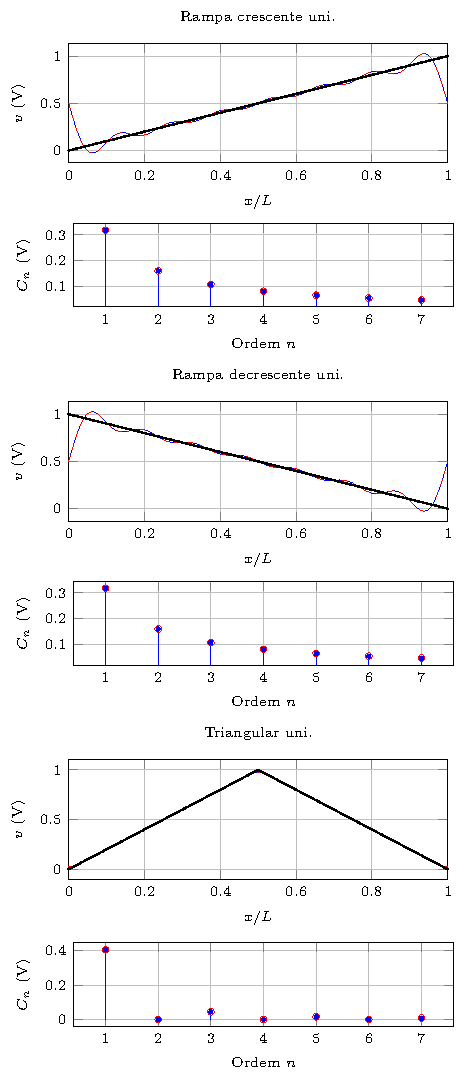
\includegraphics[width=\linewidth,height=0.86\textheight,keepaspectratio]{resultados/figuras/comparacao_basicas_unipolares.pdf}
\caption{Sinais 1 a 3 da Figura 1: ondas unipolares. Para cada sinal, apresentam-se a onda e seu espectro. Preto: amostras; azul: teoria até a ordem 7; vermelho: FFT da simulação.}\label{fig:comparacao1}
\end{figure}
\begin{figure}[H]
\centering
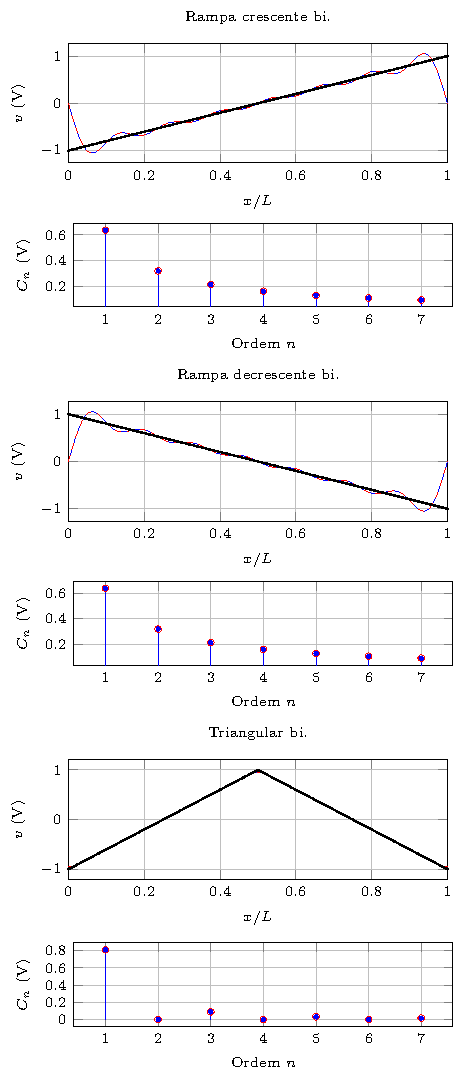
\includegraphics[width=\linewidth,height=0.86\textheight,keepaspectratio]{resultados/figuras/comparacao_basicas_bipolares.pdf}
\caption{Sinais 4 a 6 da Figura 1: ondas bipolares. Para cada sinal, apresentam-se a onda e seu espectro. Preto: amostras; azul: teoria até a ordem 7; vermelho: FFT da simulação.}\label{fig:comparacao2}
\end{figure}
\begin{figure}[H]
\centering
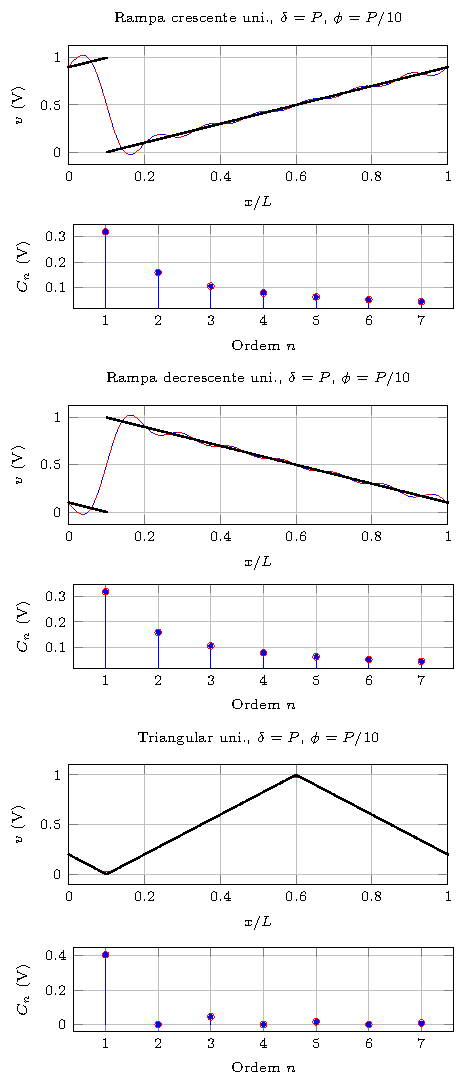
\includegraphics[width=\linewidth,height=0.86\textheight,keepaspectratio]{resultados/figuras/comparacao_deslocadas_P_unipolares.pdf}
\caption{Ondas unipolares deslocadas, $\delta=P$. Para cada sinal, apresentam-se a onda e seu espectro. Preto: amostras; azul: teoria até a ordem 7; vermelho: FFT da simulação.}\label{fig:comparacao3}
\end{figure}
\begin{figure}[H]
\centering
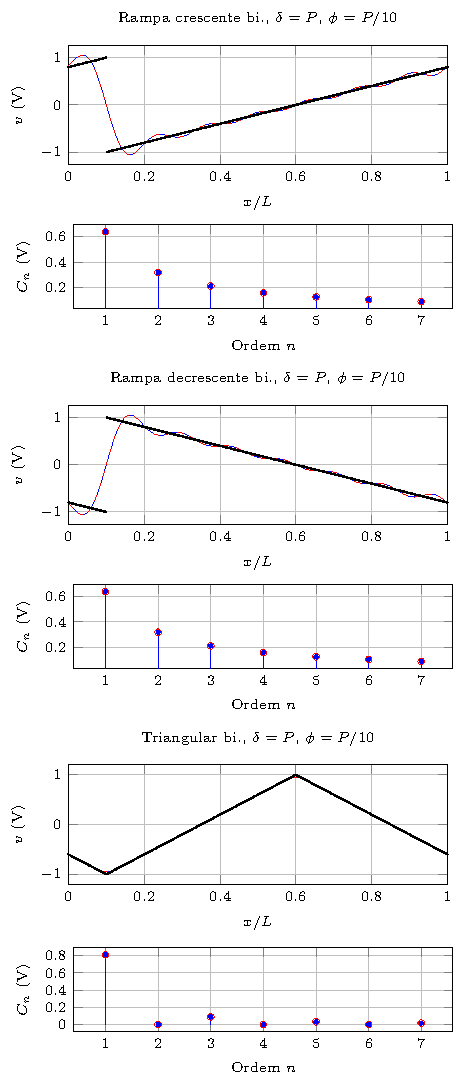
\includegraphics[width=\linewidth,height=0.86\textheight,keepaspectratio]{resultados/figuras/comparacao_deslocadas_P_bipolares.pdf}
\caption{Ondas bipolares deslocadas, $\delta=P$. Para cada sinal, apresentam-se a onda e seu espectro. Preto: amostras; azul: teoria até a ordem 7; vermelho: FFT da simulação.}\label{fig:comparacao4}
\end{figure}
\begin{figure}[H]
\centering
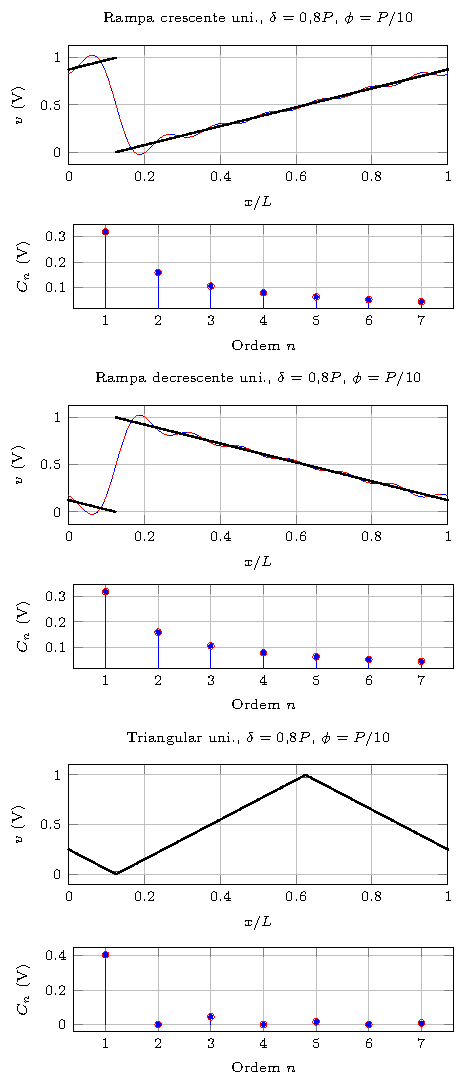
\includegraphics[width=\linewidth,height=0.86\textheight,keepaspectratio]{resultados/figuras/comparacao_deslocadas_08P_unipolares.pdf}
\caption{Ondas unipolares deslocadas, $\delta=0{,}8P$. Para cada sinal, apresentam-se a onda e seu espectro. Preto: amostras; azul: teoria até a ordem 7; vermelho: FFT da simulação.}\label{fig:comparacao5}
\end{figure}
\begin{figure}[H]
\centering
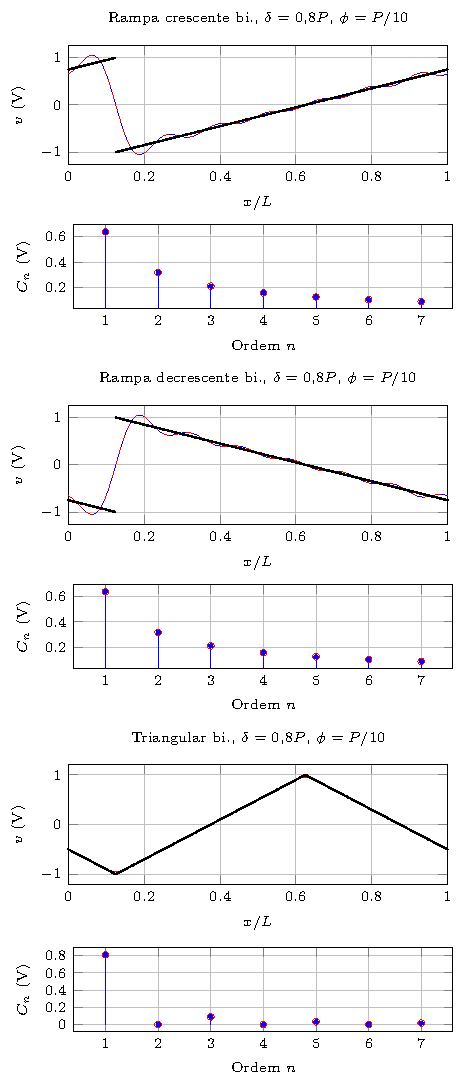
\includegraphics[width=\linewidth,height=0.86\textheight,keepaspectratio]{resultados/figuras/comparacao_deslocadas_08P_bipolares.pdf}
\caption{Ondas bipolares deslocadas, $\delta=0{,}8P$. Para cada sinal, apresentam-se a onda e seu espectro. Preto: amostras; azul: teoria até a ordem 7; vermelho: FFT da simulação.}\label{fig:comparacao6}
\end{figure}
\begin{figure}[H]
\centering
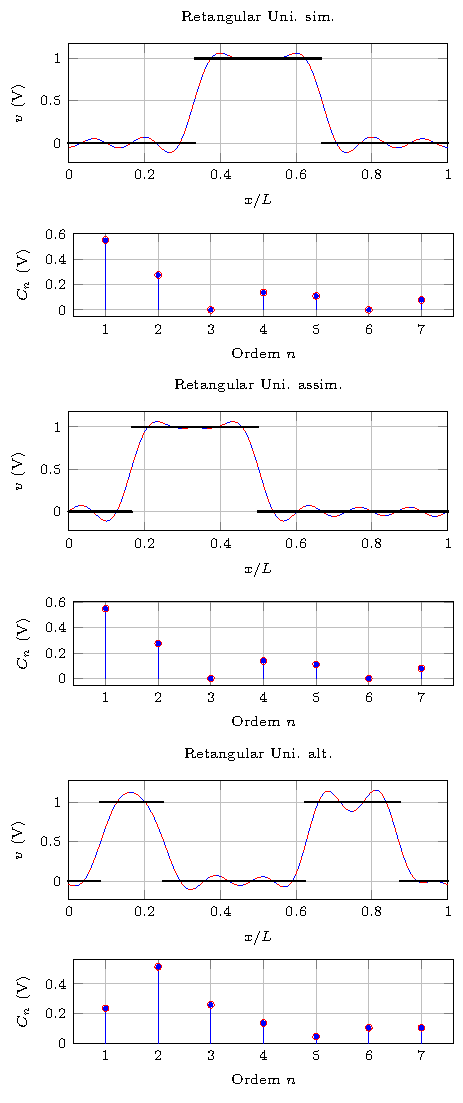
\includegraphics[width=\linewidth,height=0.86\textheight,keepaspectratio]{resultados/figuras/comparacao_retangulares_unipolares.pdf}
\caption{Retangulares unipolares: casos simétrico, assimétrico e alternado. Para cada sinal, apresentam-se a onda e seu espectro. Preto: amostras; azul: teoria até a ordem 7; vermelho: FFT da simulação.}\label{fig:comparacao7}
\end{figure}
\begin{figure}[H]
\centering
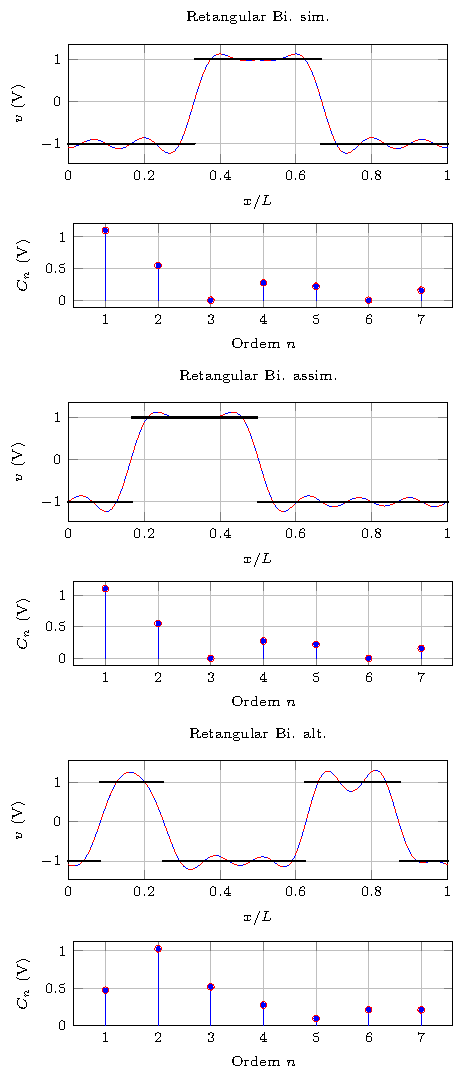
\includegraphics[width=\linewidth,height=0.86\textheight,keepaspectratio]{resultados/figuras/comparacao_retangulares_bipolares.pdf}
\caption{Retangulares bipolares: casos simétrico, assimétrico e alternado. Para cada sinal, apresentam-se a onda e seu espectro. Preto: amostras; azul: teoria até a ordem 7; vermelho: FFT da simulação.}\label{fig:comparacao8}
\end{figure}

\FloatBarrier


% 8. Análises dos Resultados
\section{Análise dos resultados}

As rampas apresentam amplitudes harmônicas proporcionais a $1/n$,
enquanto os triângulos têm decaimento proporcional a $1/n^2$ e
coeficientes pares nulos. Assim, a mesma ordem máxima 7 aproxima
melhor as ondas triangulares, já que os valores tendem a ser menores. No triângulo bipolar, a fundamental
contém aproximadamente $98{,}5534\%$ da energia; com as ordens até 7,
essa fração sobe para $99{,}9689\%$.

Nas rampas e no triângulo unipolar, a média $A/2$ representa
$75\%$ da energia total. Dessa forma, a rampa unipolar tem apenas
$22{,}9766\%$ nas ordens 1 a 7, embora a reconstrução que inclui
a média retenha $97{,}9766\%$.

Além disso, mover uma retangular dentro de um período, mantendo $D$, altera
$a_n$, $b_n$ e a fase, mas não $C_n$ nem as energias harmônicas.
Os casos simétrico e assimétrico confirmam essa propriedade.
A retangular bipolar só possui média zero para $D=1/2$; nos exemplos
com $D=1/3$, sua média é $-A/3$.

As seis ondas deslocadas obedecem à mesma invariância de energia.
Já alterar $\delta$ modifica a posição das linhas em hertz:
os exemplos de 60 e 75 Hz precisam de janelas de duração $1/60$ e
$1/75$ s, respectivamente. Usar o período nominal $P$ para analisar
uma onda com período efetivo diferente pode causar vazamento
espectral e comparar frequências que não representam as mesmas ordens.

Na alternância dos dois pulsos, o intervalo repetido é $2P$ e a
fundamental do exemplo passa a 30 Hz. A fração de energia nessa
ordem cai para $6{,}6934\%$ no unipolar e $11{,}1557\%$ no bipolar.

As reconstruções com saltos apresentam oscilações próximas às
descontinuidades, associadas ao fenômeno de Gibbs. Esse erro de
truncamento é diferente do pequeno erro da FFT amostrada em relação
aos coeficientes analíticos.






% 9. Conclusões
\section{Conclusão}

As séries de Fourier foram verificadas nos 24 cenários, com sete
pares de coeficientes por caso. A FFT das amostras geradas no
Simulink apresentou erro máximo de $\ErroCoefMax$ V por par;
os erros relativos máximos da fundamental e da energia total
foram $\ErroCUmMax\%$ e $\ErroEnergiaMax\%$, respectivamente.
A concordância foi conferida também por integração direta das
ondas e pelo teorema de Parseval.

O triângulo bipolar concentra $98{,}5534\%$ de sua energia na
fundamental e $99{,}9689\%$ até a ordem 7. Na rampa unipolar,
a reconstrução com a média e as ordens 1 a 7 retém $97{,}9766\%$;
a média sozinha responde por $75\%$ do total. O
$\mathrm{THD}_7$ de $11{,}9842\%$ dos triângulos, frente a
$71{,}5400\%$ das rampas, quantifica a menor participação relativa
dos harmônicos superiores nas ondas triangulares.

Por fim, notou-se que ao deslocar a onda a amplitude é preservada e as razões de energia também.
Reduzir o período para $0{,}8P$ eleva a frequência de 60 para 75 Hz;
alternar dois ciclos distintos produz a fundamental de 30 Hz e
participações de $6{,}6934\%$ e $11{,}1557\%$ na energia dos
retangulares unipolar e bipolar. Os pequenos erros da FFT são
compatíveis com a discretização adotada; as oscilações junto aos
saltos nas reconstruções decorrem do truncamento da série.


% 11. Anexos
%\input{Capitulos/anexos}

\end{document}
